\documentclass[12pt,letterpaper]{article}

\usepackage{fancyhdr}
\pagestyle{fancy}
\fancyhf{}
\rhead{Vaja 5}
\lhead{ORS}
\setlength{\headheight}{16pt}

\usepackage[utf8]{inputenc}
\usepackage[slovene]{babel}
\usepackage[colorlinks = true, urlcolor = blue]{hyperref}

\usepackage{xcolor}
\usepackage{listings}
\usepackage{graphicx}
\graphicspath{{./images/}}
\definecolor{mGreen}{rgb}{0,0.6,0}
\definecolor{mGray}{rgb}{0.5,0.5,0.5}
\definecolor{mPurple}{rgb}{0.58,0,0.82}
\definecolor{backgroundColour}{rgb}{1,1,1}

\lstdefinestyle{CStyle}{
    backgroundcolor=\color{backgroundColour},   
    commentstyle=\color{mGreen},
    keywordstyle=\color{magenta},
    numberstyle=\tiny\color{mGray},
    stringstyle=\color{mPurple},
    basicstyle=\footnotesize,
    breakatwhitespace=false,         
    breaklines=true,                 
    captionpos=b,                    
    keepspaces=true,                 
    numbers=left,                    
    numbersep=5pt,                  
    showspaces=false,                
    showstringspaces=false,
    showtabs=false,                  
    tabsize=2,
    language=C,
    frame=none
}

\begin{document}

\begin{center}
    \textbf{\Large Protokol SPI in njegova uporaba na STM32F4 v kombinaciji s senzorjem gibanja}   
\end{center}

\section*{SPI}

Na tokratnih vajah bomo spoznali protokol Serial Peripheral Interface (SPI). To je eden izmed najbolj razširjenih protokolov za serijsko komunikacijo na kratkih razdaljah, vsaj ko se pogovorajamo na nivoju mikrokrmilnikov oziroma vgrajenih sistemov. Protokol se pogosto uporablja za komunikacijo z različnimi senzorji in aktuatorji. S pomočjo tega protokola tako lahko komuniciramo s temperaturnimi in ostalimi vremenskimi senzorji, zasloni na dotik, krmilniki za SD kartice, krmilniki za Ethernet, USB, Flash in tako dalje.

V nadaljevanju bomo najprej spoznali osnove protokola SPI ter njegov programski vmesnik v mikrokrmilniku STM32F4. Na koncu bomo spoznali še senzor gibanja, ki ga najdemo na razvojni plošči in s katerim lahko komuniciramo z omenjenim protokolom.


\subsection*{Protokol SPI}

Protokol SPI je v 80-ih letih 20. stoletja razvilo podjetje Motorola. Že iz imena vidimo, da gre za serijsko komunikacijo. To pomeni, da hkrati pošiljamo ali sprejemamo zgolj en bit. V komunikaciji bo vedno nastopal en gospodar (angl. master) in en suženj (angl. slave). Na sliki \ref{SPImasterslave} je prikazan primer vezave SPI gospodarja in treh sužnjev. V večini primerov je gospodar mikrokrmilnik, senzorji in aktuatorji pa so sužnji. Kot vidite ima vsaka suženjska naprava 4 pine:

\begin{itemize}
    \item SCLK - Serial Clock (včasih tudi SCK ali SCL) je linija po kateri gospodar pošilja uro za sinhronizacijo prenosa.
    \item MOSI - Master Out Slave In je signal na katerem gospodar (Master) pošilja in suženjske naprave (Slave) sprejemajo podatke.
    \item MISO - Master In Slave Out je signal na katerem gospodar sprejema in suženjske naprave pošiljajo podatke.
    \item SS - Slave Select (včasih tudi CS - Chip Select) je linija, s katero gospodar določi s katero suženjsko napravo se želi pogovarjati. SS signal je aktiven, ko je na liniji logična ničla (angl. active low), neaktiven pa ko je na liniji logična enica) -- ta podatek je izjemno pomemben, ko nastavljamo izhodni PIN za SS signal.
\end{itemize}

\begin{figure}[ht!]
  \centering
  \caption{Primer vezave gospodarja in sužnjev v protokolu SPI.}
  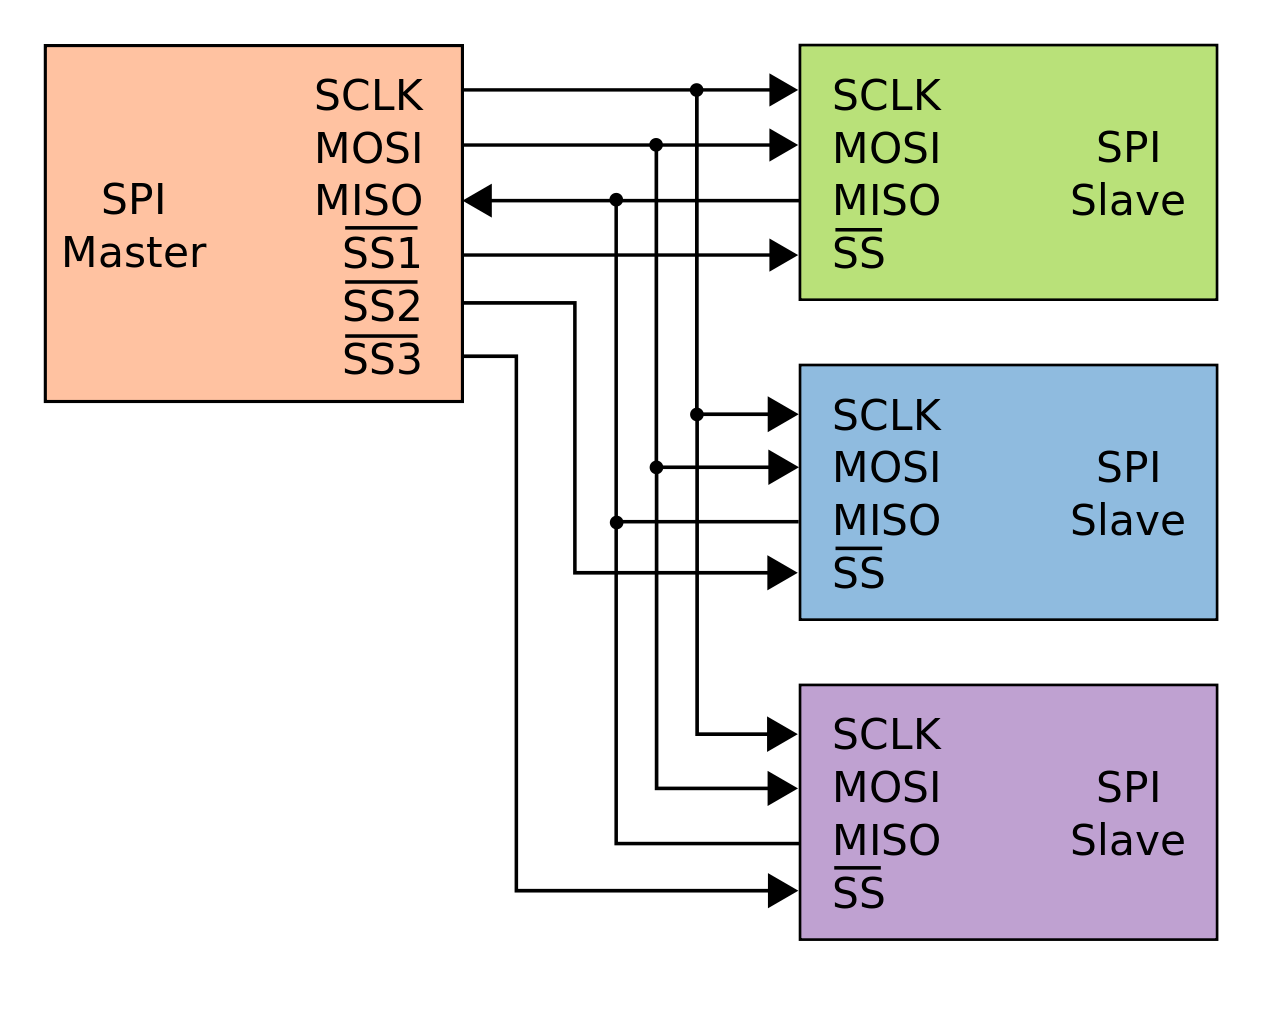
\includegraphics[width=250pt]{images/vaja5/SPI_three_slaves.png}
  \label{SPImasterslave}
\end{figure}

SPI prenos ponavadi poteka v obe smeri hkrati (angl. full duplex mode), lahko pa tudi enosmerno, kjer podatke pošilja zgolj gospodar. Gospodar je tudi tisti, ki generira urin signal, ki se pošilja hkrati s podatki. Poleg same hitrosti urinega signala ima SPI še dva parametra prenosa -- polariteto in fazo (oba parametra sta vezana na urin signal). Polariteta (CPOL) določa kašno logično vrednost ima ura v mirovanju in v katerem delu urinega signala je ura aktivna. Faza (CPHA) pa določa ob kateri urini fronti so podatki veljavni in ob kateri se spreminjajo. Na sliki \ref{SPIpolarity_phase} je prikazano obnašanje protokola SPI pri različnih nastavitvah obeh parametrov.

\begin{figure}[ht!]
  \centering
  \caption{Polariteta in faza.}
  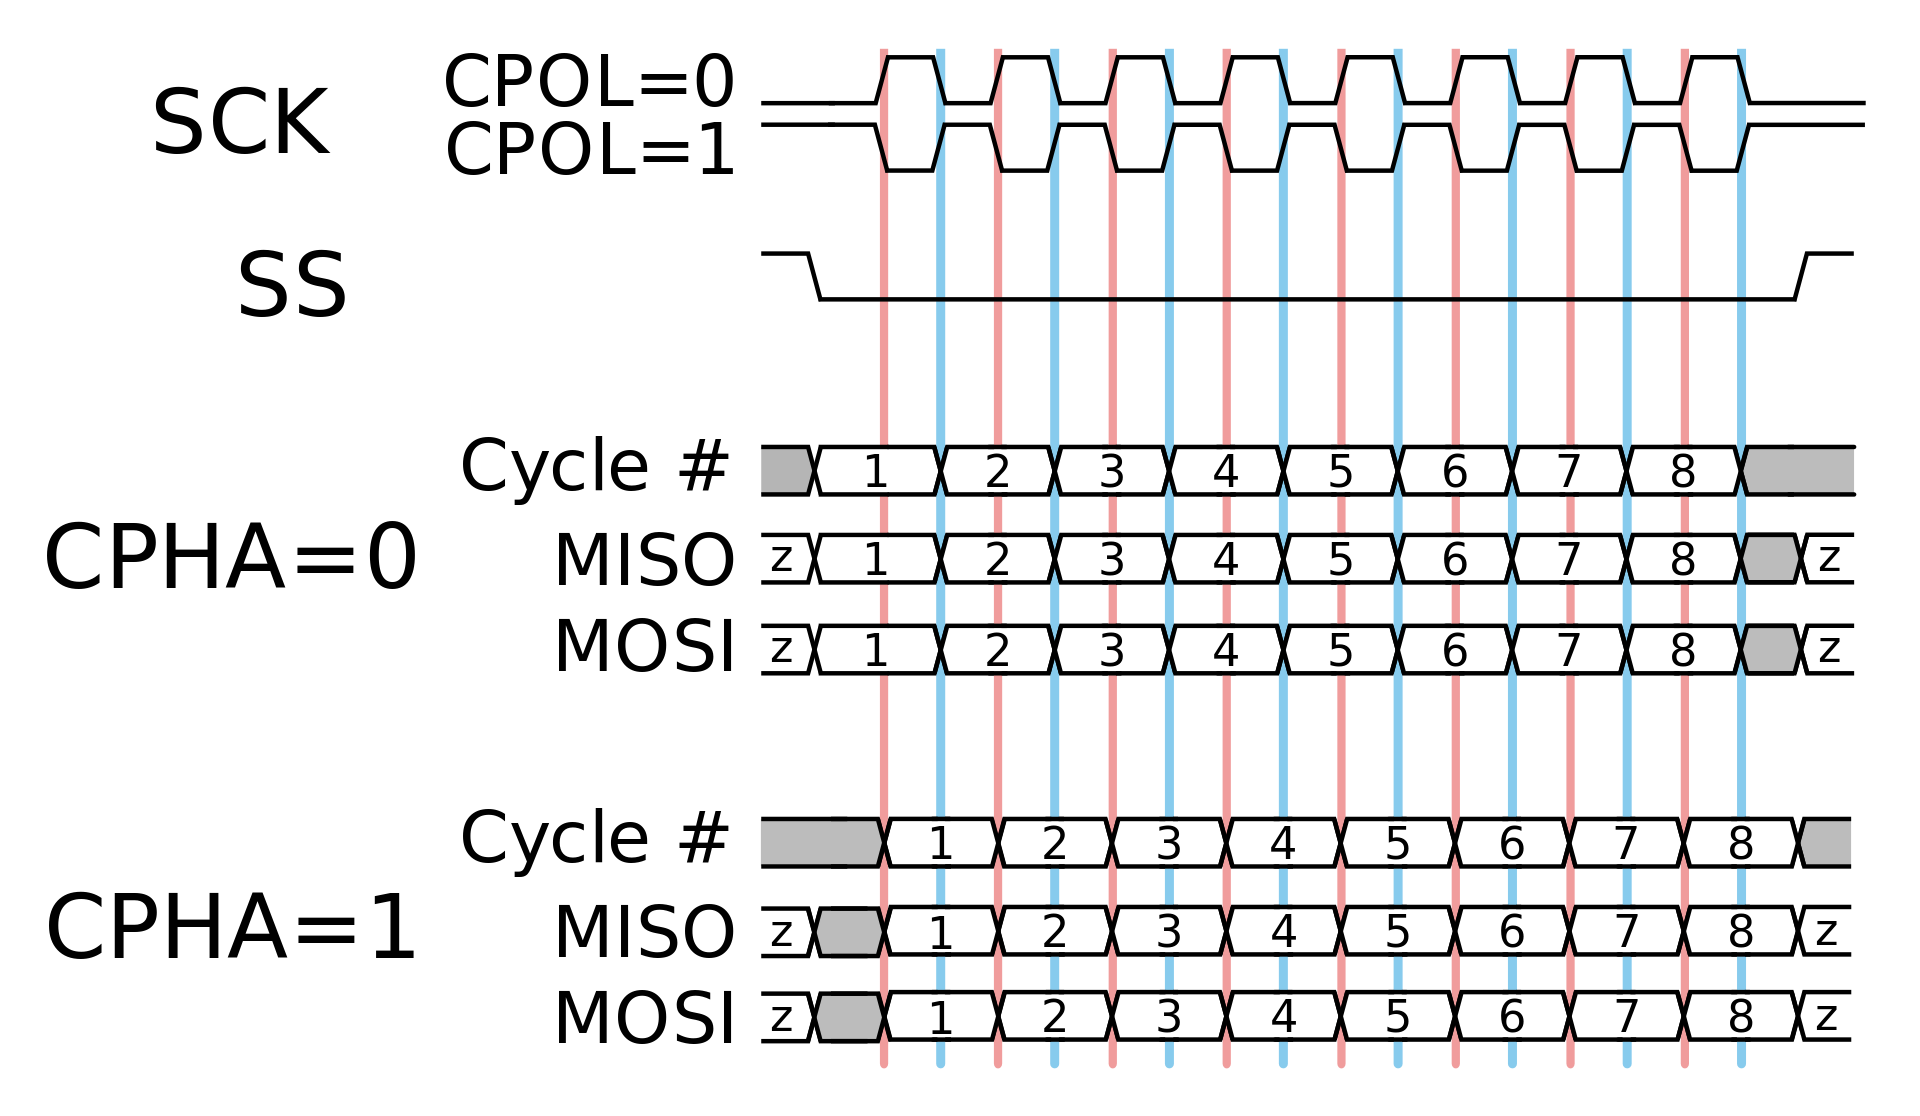
\includegraphics[width=280pt]{images/vaja5/SPI_polarity_phase.png}
  \label{SPIpolarity_phase}
\end{figure}

Zgoraj vidite, da je v primeru, ko je polariteta nič (CPOL = 0), ura, ko komunikacija ni aktivna v nizkem logičnem stanju, v primeru CPOL = 1 pa v visokem. Lahko vidite tudi, da je v primeru, ko je izbrana faza nič (CPHA = 0) posamezen bit veljaven na prvo fronto (rdeča črta), spreminja pa se na drugo fronto (modra črta). V primeru, da je CPHA = 1, pa je ravno obratno. Katero nastavitev boste nastavili SPI napravi mikrokrmilnika običajno diktirajo naprave, s katerimi želite komunicirati. SPI naprave mikrokrmilnika namreč znajo komunicirati s poljubnimi nastavitvami, enostavne in poceni suženjske naprave so tiste, ki imajo običajno omejen nabor nastavitev.

Poleg parametrov, ki so vezani na urin signal je potrebno za SPI prenos določiti še dolžino podatkov (8 ali 16 bitov), vrstni red pošiljanja bitov -- ali naj se najpomembnejši bit (angl most significant bit, MSB) pošilja prvi ali zadnji, način izbire suženjske naprave (programsko ali strojno) ter morebitna uporaba sistema CRC za preverjanje napak v prenosu. Pri slednjem moramo poleg tega ali želimo uporabiti CRC preverjanje, določiti tudi stopnjo polinom s katerim se izvede preverjanje. Tega določite številsko, konstanta $0x9$, ki jo binarno zapišemo kot $1001$ tako pomeni, da naj se uporabi CRC polinom $x^3 + x^0 = x^3 + 1$.


\subsection*{SPI v STM32F4 s knjižnico HAL}

Mikrokrmilnik STM32F407, ki ga uporabljamo na vajah, ima tri SPI naprave: SPI1, SPI2 ter SPI3. V tabeli \ref{SPIpinsTable} je zapisan seznam GPIO pinov na katere so povezani pini posameznih SPI naprav.

\begin{table}[ht!]
    \caption{Vezava pinov SPI naprav na GPIO pine.}
    \begin{center}
        \begin{tabular}{c|c|c|c}
            \textbf{Pin\textbackslash{}Naprava} & \textbf{SPI1} & \textbf{SPI2} & \textbf{SPI3} \\ \hline
            SCLK & PA5 & PB13 & PC10 \\ \hline
            MISO & PA6 & PB14 & PC11 \\ \hline
            MOSI  & PA7 & PB15 & PC12  \\
        \end{tabular}
    \end{center}
    \label{SPIpinsTable}
\end{table}

\subsubsection*{Inicializacija GPIO pinov}

GPIO pine, ki jih uporablja SPI naprava, moramo inicializirati podobno, kot smo to storili, ko smo jih inicializirali za GPIO. Glavna razlika je v tem, da jim tokrat kot način delovanja moramo določiti način alternativne funkcije (angl. alternate function). To pomeni, da s pini ne bomo upravljali mi (pisali oz. brali njihovega stanja), ampak bo pine uporabljala neka druga naprava, v tem primeru SPI. Za vsakega izmed pinov lahko uporabimo eno izmed 16 možnih alternativnih funkcij. Slika \ref{SPI_AF} prikazuje alternativne funkcije v mikrokrmilnikih STM32F407. Kot vidite, moramo v primeru, da uporabljamo SPI1 ali SPI2 pri GPIO pinih uporabiti 5. alternativno funkcijo (konstanti \texttt{GPIO\_AF5\_SPI1} in \texttt{GPIO\_AF5\_SPI2} imata vrednost \texttt{((uint8\_t)0x05)}). V primeru, da delamo z napravo SPI3 pa 6. alternativno funkcijo (konstanta \texttt{GPIO\_AF6\_SPI3} ima vrednost \texttt{((uint8\_t)0x06)}).

\begin{figure}[ht!]
  \centering
  \caption{Mapiranje alternativnih funkcij.}
  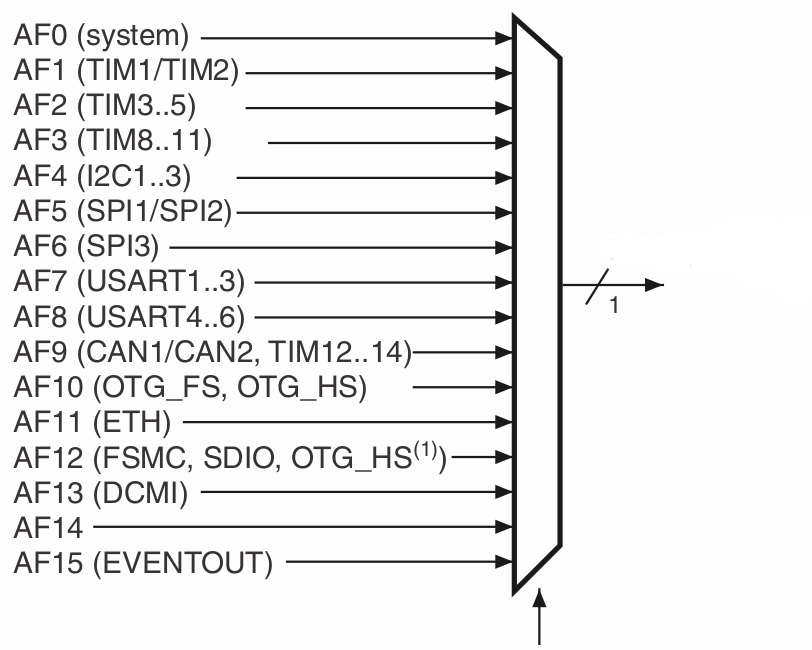
\includegraphics{images/vaja5/SPI_AF.png}
  \label{SPI_AF}
\end{figure}

\texttt{Drivers/STM32F4xx\_HAL\_Driver/Inc/stm32f4xx\_hal\_gpio\_ex.h} je datoteka, kjer najdemo seznam nastavitev za alternativne funkcije. Izsek nekaterih pomembnih vrednosti iz datoteke je prikazan spodaj.

\begin{center}
\begin{lstlisting}[style=CStyle]
#define GPIO_AF1_TIM1          ((uint8_t)0x01)
#define GPIO_AF1_TIM2          ((uint8_t)0x01)

#define GPIO_AF4_I2C1          ((uint8_t)0x04)
#define GPIO_AF4_I2C2          ((uint8_t)0x04)
#define GPIO_AF4_I2C3          ((uint8_t)0x04)

#define GPIO_AF5_SPI1          ((uint8_t)0x05)
#define GPIO_AF5_SPI2          ((uint8_t)0x05)
#define GPIO_AF5_I2S3ext       ((uint8_t)0x05)

#define GPIO_AF6_SPI3          ((uint8_t)0x06)
#define GPIO_AF6_I2S2ext       ((uint8_t)0x06)
\end{lstlisting}
\end{center}

Spodnja koda prikazuje primer inicializacije pina PB5 za uporabo v napravi SPI3. Kot vidite je inicializacija podobna kot pri klasicnih GPIO pinih, glavna in pomembna razlika je zgolj v nastavitvi alternative funkcije.

\begin{center}
\begin{lstlisting}[style=CStyle]
__HAL_RCC_GPIOB_CLK_ENABLE();

GPIO_InitTypeDef init_structure;
init_structure.Pin = GPIO_PIN_5;
init_structure.Pull = GPIO_NOPULL;
init_structure.Speed = GPIO_SPEED_FREQ_LOW;

// Mode = alternativna funkcija, obicjano nacin push-pull
// ce potrebujemo open-drain nastavimo GPIO_MODE_AF_OD
init_structure.Mode = GPIO_MODE_AF_PP;

// dolocimo se katera naprava bo upravljala s pinom
init_structure.Alternate = GPIO_AF6_SPI3;

HAL_GPIO_Init(GPIOB, &init_structure);
\end{lstlisting}
\end{center}

Pine preko katerih poteka slave select nastavimo kot običajen izhod, torej tako kot smo nastavili pine preko katerih smo prižigali LED diode.


\section*{Inicializacija SPI naprave}

Pred inicializacijo moramo podobno, kot pri GPIO napravah, prižgati uro SPI naprave. Za to uporabimo funkcije \texttt{\_\_HAL\_RCC\_SPIx\_CLK\_ENABLE()}, kjer $x$ zamenjamo z 1, 2 ali 3, odvisno katero napravo uporabljamo. Za inicializacijo SPI naprave uporabimo strukturo \texttt{SPI\_HandleTypeDef}. Prvi element strukture, ki ga bomo nastavljali je \texttt{Instance}, ki določa SPI napravo, ki jo želimo uporabiti. Možne vrednosti so \texttt{SPI1}, \texttt{SPI2} in \texttt{SPI3}.

Drugi element strukture je struktura \texttt{Init}, ki hrani vse nastavitve SPI prenosa. Posamezni elementi te strukture so opisani v nadaljevanju. Ko določimo vse nastavitve prenosa inicializiramo napravo s klicem funkcije \texttt{HAL\_SPI\_Init(*SPI\_HandleTypeDef)}.

\subsubsection*{Mode}

Nastavitev \texttt{Mode} določa ali je SPI naprava v mikrokrmilniku gospodar ali suženj, če hočemo da je naprava gospodar nastavimo parameter na vrednost\texttt{SPI\_MODE\_MASTER}, če hočemo da je suženj pa \texttt{SPI\_MODE\_SLAVE}.

\subsubsection*{Direction}

Nastavitev \texttt{Direction} določa smer prenosa.  Smer \texttt{SPI\_DIRECTION\_2LINES} pomeni, da bomo prenašali podatke v obe smeri hkrati (full-duplex), smer \texttt{SPI\_DIRECTION\_1LINE} pomeni, da bomo prenašali zgolj v eno smer. Obstaja še tretja, redko uporabljena smer \texttt{SPI\_DIRECTION\_†\_RXONLY}, s katero tako na MISO kot MOSI pinu sprejemamo podatke, torej lahko podatke prejemamo z dvakratno hitrostjo.

\subsubsection*{DataSize}

Nastavitev \texttt{DataSize} določa velikost podatkov v prenosu. Običajen 8-bitni prenos nastavimo z \texttt{SPI\_DATASIZE\_8BIT}, medtem ko za 16-bitni prenos uporabimo \texttt{SPI\_DATASIZE\_16BIT}.

\subsubsection*{FirstBit}

Nastavitev \texttt{FirstBit} določa kateri bit se pošilja prvi v prenosu: najbolj pomemben (MSB) ali najmanj pomemben (LSB). Možni nastavitvi sta tako \texttt{SPI\_FIRSTBIT\_MSB} in \texttt{SPI\_FIRSTBIT\_LSB}.

\subsubsection*{CLKPolarity}

Nastavitev \texttt{CLKPolarity} določa polariteto ure. Polariteto nič dobimo z nastavitvijo \texttt{SPI\_POLARITY\_LOW}, polariteto ena pa z \texttt{SPI\_POLARITY\_HIGH}.

\subsubsection*{CLKPhase}

Nastavitev \texttt{CLKPhase} določa fazo ure. V primeru, da so podatki veljavni na prvo fronto, spreminjajo pa se na zadnjo, nastavimo \texttt{SPI\_PHASE\_1EDGE}. Obratno situacijo dobimo z \texttt{SPI\_PHASE\_2EDGE}.

\subsubsection*{NSS}

Nastavitev \texttt{NSS} določa način dela s Slave Select (SS) pinom. Običajno s SS pinom delamo programsko kot klasičnim izhodnim pinom, ta način bomo uporabljali tudi mi, izberemo ga z vrednostjo \texttt{SPI\_NSS\_SOFT}. Druga možnost je, da s SS pinom upravlja sama SPI naprava, v tem primeru izberemo nastavitev \texttt{SPI\_NSS\_HARD\_INPUT} ali \texttt{SPI\_NSS\_HARD\_OUTPUT}.

\subsubsection*{BaudRatePrescaler}

Nastavitev \texttt{BaudRatePrescaler} določa hitrost prenosa. Tako s to nastavitvijo doličimo vrednost s katero delimo frekvenco osnovne ure za SPI napravo, ki v krmilniku STM32F407 znaša 16MHz. Najvišjo hitrost dosežemo pri nastavitvi \texttt{SPI\_BAUDRATEPRESCALER\_2}, ki uro deli z 2. Najnižjo hitrost prenosa dosežemo z \texttt{SPI\_BAUDRATEPRESCALER\_256}, ki uro deli z 256. Uro lahko delimo še z vrednostmi 4, 8, 16, 32, 64 ali 128.

\subsubsection*{CRCCalculation in CRCPolynomial}

Nastavitev \texttt{CRCCalculation} vklopi ali izklopi CRC preverjanje pri prenosu. Možni vrednosti sta \texttt{SPI\_CRCCALCULATION\_ENABLE}, ki vklopi CRC preverjanje ter \texttt{SPI\_CRCCALCULATION\_DISABLE}, ki ga izklopi. V primeru uporabe prve vrednost moramo določiti še CRC polinom. Tega določa številska nastavitev v \texttt{CRCPolynomial}.


\subsubsection*{Primer inicalizacije}

Primer inicalizacije SPI naprave je prikazan spodaj, v tem primeru nastavljamo napravo SPI1.

\begin{center}
\begin{lstlisting}[style=CStyle]
// clock on
__HAL_RCC_SPI1_CLK_ENABLE();

// init
SPI_HandleTypeDef hspi1;
hspi1.Instance = SPI1;
hspi1.Init.Mode = SPI_MODE_MASTER;
hspi1.Init.Direction = SPI_DIRECTION_2LINES;
hspi1.Init.DataSize = SPI_DATASIZE_8BIT;
hspi1.Init.CLKPolarity = SPI_POLARITY_LOW;
hspi1.Init.CLKPhase = SPI_PHASE_1EDGE;
hspi1.Init.NSS = SPI_NSS_SOFT;
hspi1.Init.BaudRatePrescaler = SPI_BAUDRATEPRESCALER_256;
hspi1.Init.FirstBit = SPI_FIRSTBIT_MSB;
hspi1.Init.CRCCalculation = SPI_CRCCALCULATION_DISABLE;
hspi1.Init.CRCPolynomial = 10;
HAL_SPI_Init(&hspi1);
\end{lstlisting}
\end{center}


\subsection*{SPI Branje in pisanje}

Ko je naprava SPI inicializirana, je pripravljena na uporabo. Če je mikrokrmilnik gospodar, moramo pred začetkom komunikacije vedno aktivirati Slave Select (SS) signal. To storimo tako, da izhodni pin postavimo na ničlo (enica na pinu SS pomeni, da je suženj deaktiviran, ničla pa da je aktiviran). Po zaključku komunikacije moramo SS signal tudi deaktivirati.

Po aktivaciji SS signala gospodar, ki dela v načinu full-duplex, začne prenos s funkcijo \texttt{HAL\_SPI\_TransmitReceive}, ki pošlje in prejme N bajtov. Prvi parameter je kazalec na inicializacijsko strukturo SPI naprave. Sledita kazalca na spremenljivke za pošiljanje in sprejemanje podatkov. Zadnja dva parametra določata število bajtov v prenosu ter maksimalni čas prenosa (angl. timeout), čas prenosa je podan v milisekundah. V primeru, da je prenos zaključen znotraj maksimalnega dovoljenega časa, funkcija vrne \texttt{HAL\_OK}, v nasprotnem primeru pa \texttt{HAL\_TIMEOUT}. Primer uporabe omenjene funkcije je prikazan spodaj. Hkrati je v spodnjem primeru prikazana še uporaba ločenih funkcij za pošiljanje za sprejemanje.

\begin{center}
\begin{lstlisting}[style=CStyle]
#define DATA_LENGTH 7
uint8_t input[DATA_LENGTH];
uint8_t output[DATA_LENGTH];

// HAL_MAX_DELAY je najvecja mozna nastavitev za timeout
HAL_SPI_TransmitReceive(&hspi1, output, input,
                        DATA_LENGTH, HAL_MAX_DELAY);

HAL_SPI_Transmit(&hspi1, output, DATA_LENGTH, HAL_MAX_DELAY);
HAL_SPI_Receive(&hspi1, input, DATA_LENGTH, HAL_MAX_DELAY);
\end{lstlisting}
\end{center}


\section*{Senzor gibanja LIS302DL}

SPI protokol bomo preizkusili v praksi na senzorja gibanja LIS302DL, ta senzor je namreč že integriran na naše razvojne plošče. SS senzorja gibanja je povezan na \textbf{GPIO pin PE3}, torej bomo za aktiviranje in deaktiviranje sužnja uporabljali ta pin! Senzor omogoča zaznavanje pospeškov do 8g, omogoča zaznavanje prostega pada in ostalih dogodkov vezanih na pospeške (``single-click'', ``double-click'', itd). Na vaji bomo spoznali le toliko, kot bomo potrebovali za izvedbo vaje. V primeru, da vas zanima več podrobnosti, si jih lahko pregledate v \href{https://www.st.com/content/ccc/resource/technical/document/application_note/e9/75/73/ca/41/5c/42/14/CD00098549.pdf/files/CD00098549.pdf/jcr:content/translations/en.CD00098549.pdf}{dokumentaciji}.

Vse nastavitve in podatke senzor gibanja hrani v 64 bajtih (registrih), do katerih želimo dostopati. V nekatere registre bomo želeli pisati, večinoma pa bomo vsebino registrov brali. Vsaka komunikacija s senzorjem je razdeljena v dva dela. V prvem delu pošljemo posebno obliko naslova registra, ki nas zanima, nato pa v drugem delu pošljemo vrednost, ki jo želimo v register vpisati ali pa preberemo vrednost registra, če želimo register prebrati.

Posebna oblika naslova je prikazana na sliki \ref{reg_LIS302DL}. Spodnjih 6 bitov določa dejanski naslov registra (0 do 63). Z RW bitom določimo, če želimo iz registra brati (RW = 1) ali v register pisati (RW = 0). Bit MB (multi byte) postavimo na 1, če nas zanima več zaporednih registrov z začetkom na podanem naslovu.

\begin{figure}[ht!]
  \centering
  \caption{Struktura naslova LIS302DL.}
  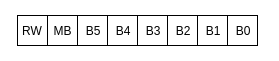
\includegraphics{images/vaja5/lis302DL.png}
  \label{reg_LIS302DL}
\end{figure}

Spodaj je prikazan primer pisanja vrednosti 0x55 na register 0x30 ter branje registra 0x31. Prikazan je tudi primer aktivacije in deaktivacije SS signala. V primeru pisanja najprej pošljemo naslov 0x30 ter nato z naslednjim ukazom še podatek, ki ga želimo vpisati. Kot vidite nam ukaz \texttt{HAL\_SPI\_TransmitReceive} pri SPI vedno vrne tudi prebrano vrednost, v primeru pisanja lahko pri obeh izvedbah ukaza vhodne podatke zavržemo, saj nas ne zanimajo.

V primeru branja najprej pošljemo naslov 0xB1 (0x31 | 0x80), 0x31 je naslov iz katerega bomo brali, bralni način pa nastavimo s postavitvijo RW bita na 1 (| 0x80). Podatek, ki ga prejmemo po izvedbi prvega ukaza \texttt{HAL\_SPI\_TransmitReceive} lahko zavržemo, saj nas ne zanima. Z naslednjim ukazom preberemo vrednost registra, ki nas je zanimal. V tem primeru pošljemo 0. V vsakem full-duplex SPI prenosu namreč moramo poslati znak če želimo znak tudi prejeti. Temu pristopu rečemo slepo pisanje (angl. blind write). Vhodnega podatka v tem primeru ne zavržemo, saj je bilo branje tega podatka naš cilj.

\begin{center}
\begin{lstlisting}[style=CStyle]
uint8_t in; // variable for dummy in data
uint8_t out; // variable for out data
uint8_t data; // variable for in data

// WRITE EXAMPLE
// slave select
HAL_GPIO_WritePin(GPIOE, GPIO_PIN_3, GPIO_PIN_RESET);
// set address
out = 0x30;
HAL_SPI_TransmitReceive(&hspi1, &out, &in, 1, HAL_MAX_DELAY);
// write data
out = 0x55;
HAL_SPI_TransmitReceive(&hspi1, &out, &in, 1, HAL_MAX_DELAY);
// slave deselect
HAL_GPIO_WritePin(GPIOE, GPIO_PIN_3, GPIO_PIN_SET);

// READ EXAMPLE
// slave select
HAL_GPIO_WritePin(GPIOE, GPIO_PIN_3, GPIO_PIN_RESET);
// set address 0x31, and read mode or with 0x80
out = 0x31 | 0x80;
HAL_SPI_TransmitReceive(&hspi1, &out, &in, 1, HAL_MAX_DELAY);
// read data
out = 0x0;
HAL_SPI_TransmitReceive(&hspi1, &out, &data, 1, HAL_MAX_DELAY);
// read value is now stored in data variable!

// slave deselect
HAL_GPIO_WritePin(GPIOE, GPIO_PIN_3, GPIO_PIN_SET);
\end{lstlisting}
\end{center}

Za vklop osnovnega merjenja pospeškov moramo v LIS302DL na naslov 0x20 zapisati vrednost 0x47! Po vklopu merjenja je priporočljivo, da s senzorjem vsaj 100 milisekund ne komuniciramo, saj senzor potrebuje nekaj časa da se zažene in stabilizira.

V tokratni nalogi nas bo zanimal naklon razvojne plošče po x in y osi. Prvega dobimo tako, da preberemo register na naslovu 0x29, drugega pa na naslovu 0x2B. Obe vrednosti sta 8-bitni predznačeni števili, ki imata vrednosti blizu 0, ko je razvojna plošča poravnana (npr. na ravni mizi).

\newpage

\subsection*{Priprava projekta}

Za to, da lahko uporabimo SPI funkcije moramo v projekt v STM32Cube dodati datoteke iz STM32 HAL knjižnice. Vse datoteke knjižnice se nahajajo na:

\begin{itemize}
    \item Windows:
    
    \texttt{C:/Users/<username>/Repository/STM32Cube\_FW\_F4\_V1.24.1\\/Drivers/STM32F4xx\_HAL\_Driver}
    
    \item Unix:
    
    \texttt{/home/username/STM32Cube/}
\end{itemize}


Za uporabo SPI funkcij kopirajte datoteko \texttt{Src/stm32f4xx\_hal\_spi.c} iz knjižnice v projekt na lokacijo \texttt{Drivers/STM32F4xx\_HAL\_Driver/Src}.

Nato skopirajte še datoteko \texttt{Inc/stm32f4xx\_hal\_spi.h} iz knjižnice v projekt na lokacijo \texttt{Drivers/STM32F4xx\_HAL\_Driver/Inc}.

Ko dodate datoteki, v \texttt{Inc/stm32f4xx\_hal\_conf.h} odkomentirajte vrstico, ki definira \texttt{HAL\_SPI\_MODULE\_ENABLED}. Obe datoteki lahko najdete tudi na spletni učilnici, pri gradivu za vajo 5.

\newpage

\section*{Naloga}

Pri tokratni nalogi boste realizirali digitalno vodno tehtnico, ki ji po domače bolj pogosto rečemo vaservaga. Spodaj so označene 4 LED diode, ki jih imamo na razvojni plošči. Napišite program, ki bo v primeru, da je plošča nagnjena v smeri LED diode D, prižgala LED B in obratno prižgala LED D, ko bo plošča nagnjena v smeri LED B. Podobno realizirajte tudi v smeri LED diod A in C. V primeru, da je razvojna plošča poravnana, ugasnite vse 4 LED diode.

\begin{figure}[ht!]
  \centering
  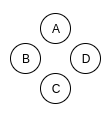
\includegraphics{images/vaja5/led.png}
  \label{LIS302DL}
\end{figure}

Kot smo že zapisali v poglavju o senzorju gibanja, je Slave Select senzorja povezan na GPIO pin PE3. MISO, MOSI in SCLK pini senzorja gibanja so povezani na pine PA5, PA6 ter PA7 naprave SPI1.

\end{document}
